\section{Photometric redshifts}
\label{sec:photoz}

We will perform the galaxy clustering study in several photometric redshift (photo-z) bins. Therefore, we will need to estimate the photo-z of each galaxy in the Mega-Z sample. Furthermore, the theoretical predictions for the clustering need the true-redshift distribution of the galaxies in each photo-z bin $i$, $N_i(z)$, which we can obtain from the 2SLAQ sample. 
For this purpose, we need to compute photometric redshifts of the 2SLAQ galaxies, split them into several photo-z bins, and, finally, recover the spectroscopic redshift distribution in each bin. Additionally, we will study the photo-z performance using 2SLAQ, and apply photo-z quality cuts to improve it. The impact of these cuts on $N_i(z)$ will also be studied.

We use the Bayesian Photometric Redshifts\footnote{\texttt{BPZ} can be found at \url{http://www.its.caltech.edu/~coe/BPZ/}.} (BPZ) template-fitting code described in~\citet{Benitez2000} to compute the photometric redshift of galaxies in both catalogs. It uses Bayesian statistics to produce a posterior probability density function $p(z|m_i)$ that a galaxy is at redshift $z$ when its magnitudes are $m_i$:
\begin{equation}
p(z|m_i) \propto \sum_t L(m_i|z,t) \, \Pi(z,t \mid m_i)  \, ,
\label{pz}
\end{equation} 
where $L(m_i|z,t)$ is the likelihood that the galaxy has magnitudes $m_i$, if its redshift is $z$ and its spectral type $t$, and $\Pi(z,t \mid m_i)$ is the prior probability that the galaxy has redshift $z$ and spectral type $t$. Finally, the photometric redshift $z(phot)$ of the galaxy will be taken as the position of the maximum of $p(z|m_i)$.

Each spectral type $t$ can be represented by a galaxy template. BPZ includes its own template library, but we prefer to use the new \texttt{CWW} library from \texttt{LePhare}\footnote{The new \texttt{CWW} library can be found in the folder \tt{/lephare\_dev/sed/GAL/CE\_NEW/} of the \texttt{LePhare} package at \url{http://www.cfht.hawaii.edu/~arnouts/LEPHARE/DOWNLOAD/lephare\_dev\_v2.2.tar.gz}.}, another template-based photo-z code described in \citet{Arnouts1999,Ilbert2006}. Both libraries are based on \citet{Coleman1980,Kinney1996}, but \texttt{BPZ} contains only 8 templates compared to 66 in~\texttt{LePhare}. The large number of templates allows us to focus on the LRG templates, which correspond to the genuine galaxy type of our catalogs. In particular, we select four: \texttt{Ell\_01}, \texttt{Ell\_09}, \texttt{Ell\_19} and \texttt{Sbc\_06}, and then we create nine interpolated templates between consecutive templates, giving a total of 31 templates, shown in Fig.~\ref{2slaq_templates}.

\begin{figure}
\centering
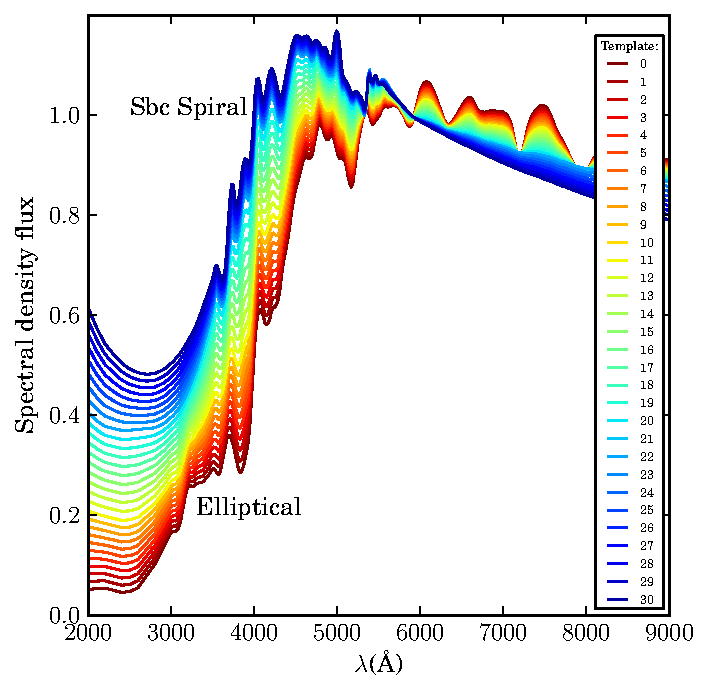
\includegraphics[type=pdf,ext=.pdf,read=.pdf, width=80mm]{./plots/2slaq_templates}
\caption{The spectral galaxy templates used in the determination of the 2SLAQ and Mega-Z photo-zs. There are a total of 31 templates that range from elliptical galaxies, the vast majority in both samples, to Sbc spiral galaxies.}
\label{2slaq_templates}
\end{figure}
Template-based photo-z codes require the knowledge of the filter band-passes of the survey instrument in order to compute the predicted photometry that will be compared with the observations to produce the likelihood $L(m_i|z,t)$. The SDSS instrument carries five broad-band filters, \textit{ugriz}, described in \citet{Fukugita1996}, whose throughputs are obtained from~\url{http://home.fnal.gov/~annis/astrophys/filters/filters.new}.

A crucial point of \texttt{BPZ} is the prior probability $\Pi(z, t \mid m)$ that helps improve the photo-z performance. \citet{Benitez2000} proposes the following empirical function:
\begin{equation}
\Pi(z, t \mid m) \propto f_t e^{-k_t(m-m_0)} \cdot z^{\alpha_t}\exp \left\lbrace -\left[ {z \over z_{mt}(m)} \right]^{\alpha_t} \right\rbrace,
\label{prior}
\end{equation}
where $z_{mt}(m) = z_{0t} + k_{mt}(m-m_0)$. Every spectral type $t$ has associated a set of five parameters $\lbrace f,k,\alpha,z_0,k_{m} \rbrace$ that determine the shape of the prior. These parameters are determined from the spectroscopic data themselves. In principle, we could assign one prior $\Pi(z, t \mid m)$ to each one of the 31 templates in Fig.~\ref{2slaq_templates}, but this would give a total of $31\times5=155$ parameters, too many for the spectroscopic data sample available. Instead, we split the 31 templates in two groups: $t=1$, with the 10 first templates that make up the group of pure elliptical galaxies, and $t=2$ with the rest. Then, running \texttt{BPZ} on 2SLAQ a first time, without priors, we find the group each galaxy belongs to. Fitting~(\ref{prior}) to this output, together with the spectroscopic redshifts and the observed magnitudes in one band (we choose the $i$ band), we find the values of the prior parameters. Results are given in Table~\ref{tab:prior}.
\begin{table}
\centering
\begin{tabular}{cccccc}
\hline
$t$ & $f$ & $k$ & $\alpha$ & $z_0$ & $k_{m}$ \\ \hline
1 & 0.72 & 0.0 & 8.679 & 0.477 & 0.078\\
2 & 0.14 & 0.0 & 7.155 & 0.488 & 0.064\\
\hline
\end{tabular}
\caption{The values of the prior parameters of (\ref{prior}) for the 2SLAQ galaxies.}
\label{tab:prior}
\end{table}

The $k$ parameters are related to the migration of galaxies from one spectral type to another at different magnitudes. The fit gives values of $k$ very close to 0, so we impose explicitly not having type migration by setting them exactly to 0. $f$ gives the fraction of galaxies of each type at magnitude $m_0$, which we choose to be $m_0=18.5$. Since $k=0$, we find that the 72\% of the galaxies belong to the spectral type group 1 independently of the magnitude, confirming that most of the galaxies are purely elliptical.

We define galaxies with catastrophic redshift determinations as those with $|\Delta z| \equiv |z(phot) - z(spec)| > 1$, where $z(spec)$ is the spectroscopic redshift and $z(phot)$ the photo-z. With the help of the prior, we are able to remove all these catastrophic redshift determinations, which account for $\sim$4.2\% of the 2SLAQ sample. They are typically galaxies with degeneracies in their color space, which cause confusions in the template fit and result in a photo-z much larger than the real redshift. Defining the photo-z precision $\sigma_z$ as half of the symmetric interval that encloses the 68\% of the $\Delta z$ distribution area around the maximum, we also find that its value for the non-catastrophic determinations improves by a factor 1.7, down to $\sigma_z \sim0.042$, in agreement with \citet{Padmanabhan2005,Collister2007,Thomas2011b}.

We also apply a cut on the quality of the photometry, consisting of not using any band, for each galaxy, with magnitude error $>$0.5. This cut mostly removes the information from the \textit{u} band for many galaxies, since the signal-to-noise tends to be lower in this band. The overall precision improves slightly to $\sigma_z \sim0.041$.

Photo-z codes, besides returning the best estimate for the redshift, typically also return an indicator of the photo-z quality. It can be simply an estimation of the error on $z(phot)$, or something more complex, but the aim is the same. In \texttt{BPZ}, this indicator is called \textit{odds}, and, it is defined as
\begin{equation}
odds = \int^{z(phot)+\delta z}_{z(phot)-\delta z}p(z|m_i)dz \, ,
\label{odds}
\end{equation} 
where $\delta z$ determines the redshift interval where the integral is computed. \textit{Odds} can range from 0 to 1, and the closer to 1, the more reliable is the photo-z determination, since $p(z|m_i)$ becomes sharper and most of its area is enclosed within $z(phot)\pm \delta z$. In our case, we choose $\delta z = 0.03$, which is close to the photo-z precision in 2SLAQ and Mega-Z. A bad choice of $\delta z$ could lead to the accumulation of all \textit{odds} close to either 0 or 1. Since \textit{odds} are a proxy for the photo-z quality, we should expect a correlation between the \textit{odds} and $\Delta z$, in the sense that higher \textit{odds} should correspond to lower $|\Delta z|$. In Fig.~\ref{sigvseff}, we show $\sigma_z$ for subsets of the Mega-Z sample with increasingly higher cuts on the \textit{odds} parameter. In fact, the exact \textit{odds} values are quite arbitrary, since they depend on the size of $\delta z$. Therefore, we have translated these \textit{odds} cuts into the fraction of the galaxy sample remaining after a certain cut has been applied. The abcissa in Fig.~\ref{sigvseff} corresponds to this completeness for increasingly tighter \textit{odds} cuts. 
\begin{figure}
\centering
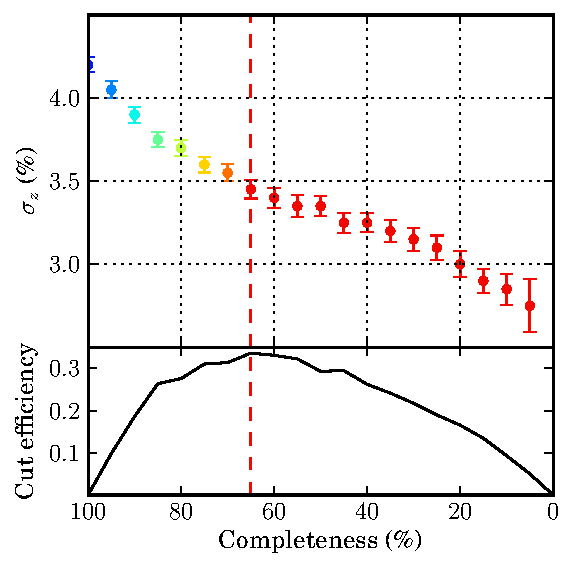
\includegraphics[type=pdf,ext=.pdf,read=.pdf, width=80mm]{./plots/sigvseff}
\caption{Top plot: the 2SLAQ photo-z precision $\sigma_{z}$ for different photo-z quality cuts resulting in the completeness shown on the $x$ axis. The error bars are computed using bootstrap~\citep{efron79}. The color scale labels the different photo-z quality cuts, here and also in Figs.~\ref{2slaq_pz_results} and \ref{Nz_bins}. The nominal precision, without any \textit{odds} cut, is 0.042. It can be improved by a factor 1.5 when the most aggressive cut, which leaves only 5\% of the galaxies, is applied. However, on the bottom plot, we see that the most efficient cut (defined in (\ref{cut_efficiency})) is at 65\% completeness, where by removing 35\% of the galaxies we achieve 50\% of the improvement, with $\sigma_z\sim0.035$. Only cuts with completeness $\geq65\%$ are considered in the following.}
\label{sigvseff}
\end{figure}

We see that, by removing the galaxies with low \textit{odds} in steps of 5\% in completeness, we are able to reduce the photo-z dispersion from $\sigma_z \sim$ 0.042 to $\sim$0.028, a factor of 1.5. Obviously, the best accuracy is obtained when the completeness is close to 0\%, but this is very inefficient. Defining the efficiency of the cut as:
\begin{equation}
\text{Cut Efficiency } (x) = x \left[ {\sigma_z (100\%) - \sigma_z(x) \over \sigma_z (100\%) - \sigma_z(0\%)} \right],
\label{cut_efficiency}
\end{equation}
where $x$ is the completeness of the catalog after the cut, we find that the most efficient photo-z quality cut is at 65\% of completeness, where $\sigma_z \sim 0.035$, as shown in the bottom plot in Fig.~\ref{sigvseff}. Since we cannot compute $\sigma_z(0\%)$ for lack of galaxies, we use instead in~(\ref{cut_efficiency})
the value at 5\% completeness. From now on, we will refer to photo-z quality cuts as all those in Fig.~\ref{sigvseff} that lead to a completeness between 100\% and 65\%, and which are labeled in different colors.

An exhaustive analysis of the photo-z results is shown in Fig.~\ref{2slaq_pz_results}. It consists of a series of plots where different statistical properties of $\Delta z$, in the rows, are shown as a function of two different variables, in the columns: $i_{deV}$ magnitude on the left, and the photo-z estimation, $z(phot)$ on the right. In the first row, we can see the $\Delta z$ scatter from which the rest of plots are derived. As in Fig.~\ref{sigvseff}, the color progression of the curves from blue to red corresponds to the different photo-z quality cuts with completeness going from 100\% to 65\%, the most efficient cut, in steps of 5\%. The number of galaxies, in the second row, grows for increasing magnitudes, but drops for increasing redshifts. The completeness, in the third row, drops at high magnitudes,
especially when quality cuts become harder. It is quite constant along redshift. The bias (median), in the forth row, shows a general offset of $\sim$ 0.02, so that photo-zs are in general $\sim$4\% larger than the actual redshift. The photo-z precision $\sigma_z$, in the fifth row, degrades slightly for fainter galaxies, while it does by a factor of almost 3 for high-z galaxies. As in Fig.~\ref{sigvseff}, the harder the photo-z quality cut, the better precision we get. Finally, the last estimator is the outlier fraction, defined as the fraction of galaxies with $|\Delta z|$ above three times $\sigma_z$. It decreases from 10\% to 3\% for increasing magnitudes, while it keeps constant around 3\% along redshift. The photo-z quality cuts help reduce it at some magnitudes and redshifts. 
\begin{figure*}
\centering
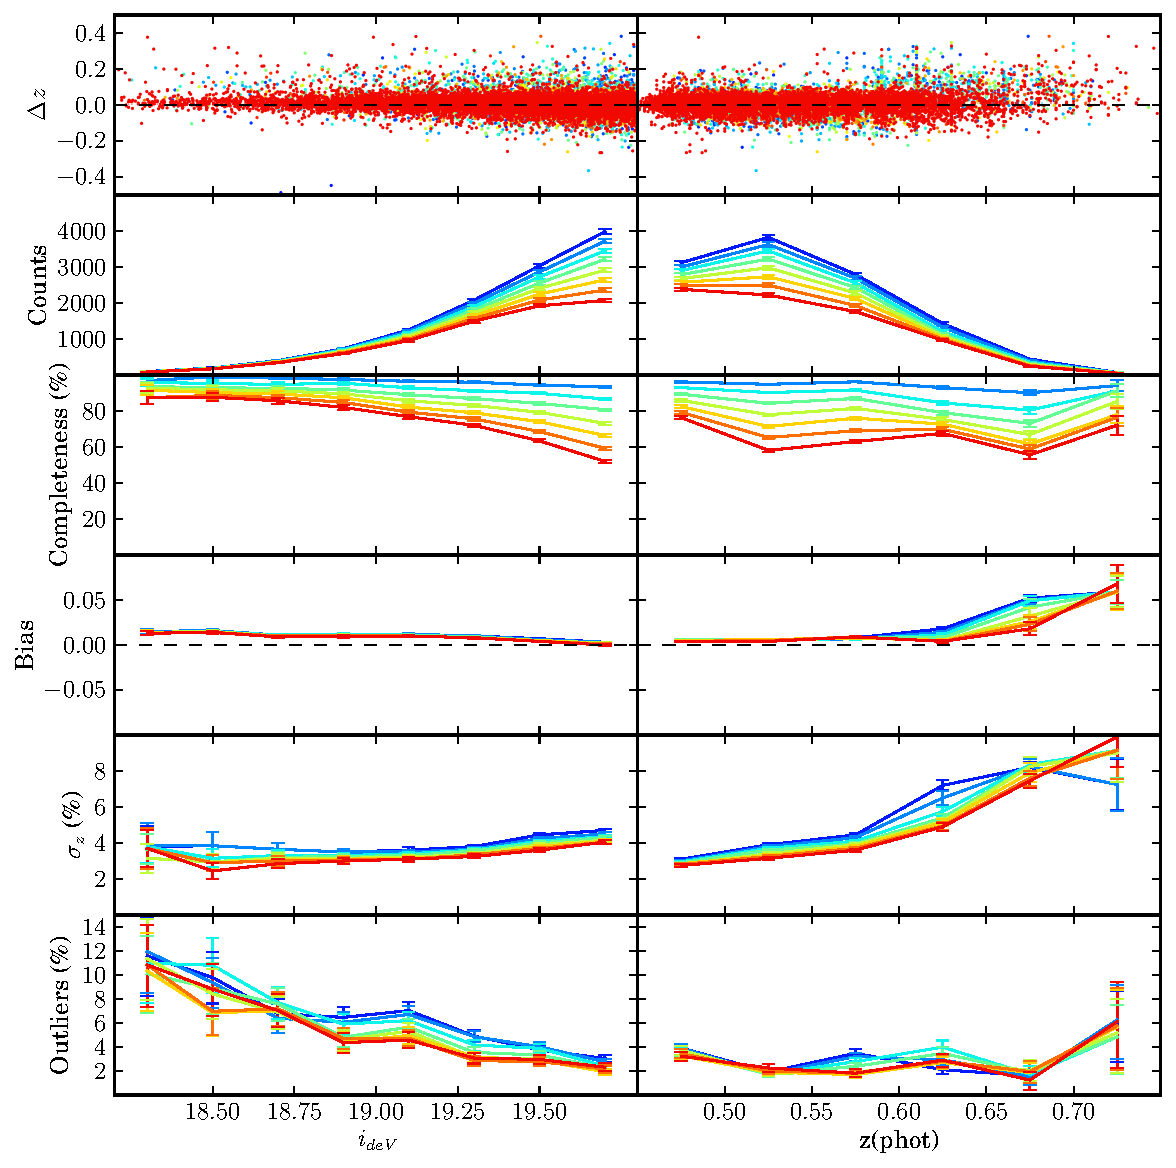
\includegraphics[type=pdf,ext=.pdf,read=.pdf, width=135mm]{./plots/2slaq_DR7}
\caption{Statistics showing the 2SLAQ photo-z performance. In the first row we show the scatter of $\Delta z \equiv z(phot) - z(spec)$ with respect to the $i_{deV}$ magnitude (left) and $z(phot)$ (right). The scatter has been binned along these two variables and some statistical estimators have been computed in each bin. In descending order of rows, we show the galaxy population (in counts), the completeness, the bias (median), the photo-z precision $\sigma_z$ and the 3$\sigma$ outlier fraction. The color degradation from red to blue is the same as in Fig.~\ref{sigvseff} and labels different photo-z quality cuts.}
\label{2slaq_pz_results}
\end{figure*}

In Fig.~\ref{Nz_megaz}, we have compared the 2SLAQ photo-z distribution with the spectroscopic redshift distribution. Both distributions are clearly different at low redshift. While the photo-z distribution rises very sharply from $z\sim0.45$, reaching the maximum immediately, the spectroscopic distribution rises much more gradually from $z\sim0.25$. This is because the color cut in (\ref{zp_cut}) acts as a photo-z cut at $z(phot)\gtrsim0.45$. Figure~\ref{Nz_megaz} also contains the photo-z distribution of the Mega-Z galaxies. It closely resembles the photo-z distribution in 2SLAQ, but they are not as similar as the magnitude distributions in Fig.~\ref{Nm_megaz}. 
\begin{figure}
\centering
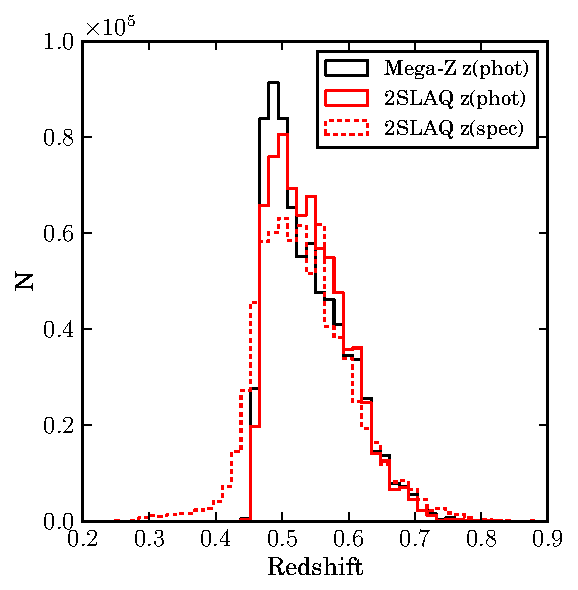
\includegraphics[type=pdf,ext=.pdf,read=.pdf, width=85mm]{./plots/Nz_megaz}
\caption{The photo-z distribution of Mega-Z (black), and the spectroscopic (red dashed) and photometric (red solid) redshift distributions of 2SLAQ. The 2SLAQ distributions have been normalized to the Mega-Z number of galaxies for comparison.}
\label{Nz_megaz}
\end{figure}

Finally, we split the 2SLAQ and Mega-Z catalogs into four photo-z bins of equal width 0.05. The width has been chosen to roughly match the photo-z precision of the catalogs. We want to know the actual redshift distributions inside each of these photo-z bins in order to make the predictions for clustering in the next section. For this purpose, we use the spectroscopic information in 2SLAQ. In Fig.~\ref{Nz_bins} we show the spectroscopic redshift distributions of these four photo-z bins in 2SLAQ at the different photo-z quality cuts of Fig.~\ref{sigvseff}, using the same color labeling. All the distributions have been normalized in order to compare them. As expected, the distributions become wider in the higher photo-z bins. This is in agreement with the increasing $\sigma_z$ with redshift seen in Fig.~\ref{2slaq_pz_results}. On the other hand, photo-z quality cuts tend to reduce the width of the distributions. For instance, the left tail of the last bin, at $0.6<z(phot)<0.65$, is drastically reduced when the most efficient photo-z quality cut is applied. 
\begin{figure}
\centering
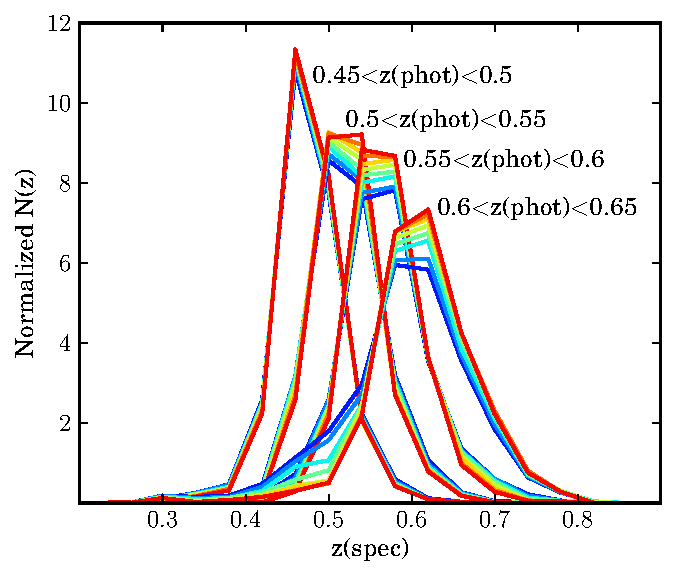
\includegraphics[width=80mm]{./plots/Nz_bins_megaz.pdf}
\caption{The spectroscopic redshift distributions in the 2SLAQ catalog for the four photo-z bins in which we will measure galaxy clustering in section~\ref{sec:clustering}. They are all normalized to the same area under the curves. Different colors label different photo-z quality cuts, as in Figs.~\ref{sigvseff} and \ref{2slaq_pz_results}.}
\label{Nz_bins}
\end{figure}
